\documentclass{standalone}
\usepackage{tikz, fkmath}
\begin{document}
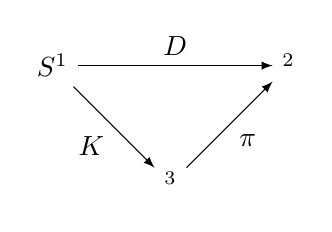
\begin{tikzpicture}
  \node (S1) at (-1.5,1) {$S^1$};
  \node (R2) at (1.5,1) {$\RR^2$};
  \node (R3) at (0,-.5) {$\RR^3$};

  \draw[-latex] (S1) -- (R2) node[above, midway] {$D$};
  \draw[-latex] (S1) -- (R3) node[below left, midway] {$K$};
  \draw[-latex] (R3) -- (R2) node[below right, midway] {$\pi$};
\end{tikzpicture}
\end{document}
